\documentclass[a4paper,12pt,oneside]{book}
\usepackage[a4paper, width=160mm, top=20mm,bottom=20mm]{geometry}
\usepackage{graphicx}
\usepackage{listings}
\usepackage[boxed]{algorithm2e}
\usepackage[final]{pdfpages}
\usepackage{multirow}
\usepackage{color}
\usepackage{amsmath}
\usepackage{hyperref}
\hypersetup{colorlinks=true}
\hypersetup{pdfborder={0 0 0}}
\author{Prakash Gautam}
\title{\Huge A\\Close Look at\\ Breshenham Algorithm\\  \small (Line Circle and Ellipse)}

\date{Jan 19, 2014}
\begin{document}
\begin{titlepage}
	\begin{center}
		\maketitle
	\end{center} 
\end{titlepage}

\pagenumbering{roman}
\tableofcontents
\vfill
\pagebreak


%Let us cee if it works

\definecolor{mygreen}{rgb}{0,0.6,0}
\definecolor{mygray}{rgb}{1.0,0.5,0.5}
\definecolor{mymauve}{rgb}{0.58,0,0.82}
\lstset{ %
morekeywords={cout,cin},
backgroundcolor=\color{white}, % choose the background color; you must add \usepackage{color} or \usepackage{xcolor}
basicstyle=\ttfamily, % the size of the fonts that are used for the code
breakatwhitespace=false, % sets if automatic breaks should only happen at whitespace
breaklines=true, % sets automatic line breaking 
%captionpos=b, % sets the caption-position to bottom
commentstyle=\color{mygreen}, % comment style
deletekeywords={...}, % if you want to delete keywords from the given language
escapeinside={\%*}{*)}, % if you want to add LaTeX within your code
extendedchars=true, % lets you use non-ASCII characters; for 8-bits encodings only, does not work with UTF-8
%frame=single, % adds a frame around the code 
keywordstyle=\color{blue}, % keyword style 
language=C++, % the language of the code
morekeywords={*,...}, % if you want to add more keywordsto the set
numbers=none, % where to put the line-numbers; possible values are (none, left, right)
numbersep=5pt, % how far the line-numbers are from the code
numberstyle=\tiny\color{mygray}, % the style that is used for theline-numbers
rulecolor=\color{black}, % if not set, the frame-color may be changed on line-breaks within not-black text (e.g. comments (green here))
showspaces=false, % show spaces everywhere adding particular underscores; it overrides ‚showstringspaces‚
showstringspaces=false, % underline spaces within strings only
showtabs=false, % show tabs within strings adding particular underscores
stepnumber=1, % the step between two line-numbers. If it‚s 1, each line will be numbered
stringstyle=\color{mymauve}, % string literal style
tabsize=2, % sets default tabsize to 2 spaces
%title=\lstname % show the filename of files included with \lstinputlisting; also try caption instead of title
%directives={include,define}
}

%Let Us really see upto this


\section*{Preface}

I really don't know what should a good preface look like, but since before reading any book one should at least go through its preface which in turn will decide whether the reader will go any further, I shall try to encourage to at least go through all the pages of this book(?).\\

This book is my attempt to try to explain what I pretend to understand. At first I thought Breshenham algorithm was just some kind of rounding off algorithm to approximate the floating point output of equation to integers to plot into the always-integer-valued pixels. But this algorithm turns out to be way more than that. It is very very simple and yet very powerful that cuts short the complex calculations needed otherwise to find the points of certain geometric shapes.\\

I don't assume that the reader has knowledge of Breshenham algorithm prior to this yet prior knowledge does no harm but help. Optional knowledge of C++ programming is good if the reader wants to use the C++ program codes given.
\\ This book is completely my original writing. Except for the Q/A I did on the class with my teacher, I've not referred any books or internet or anything. But the success of programs written and tested times and again in C++ suggest that the discussion given on the book are correct. As far as possible I've tried to explain the matter in plain language with common words. No figures  used in this book are taken from any existing source.\\

I would like to thank my friends form encouraging me to write this and their appreciation has always pushed me further. Also I shall thank my friends in the class for coping me and my rigorous questions. I would sincerely thank my teacher who suggested me to use {\LaTeX} and answered my questions in the class without any irritation. I shall thank him for his lecture in the class which introduced me to Breshenham algorithm,\\

Comments and suggestions are always welcome and are sincerely expected and accepted.
\\
\\
\textbf{Prakash Gautam}\\
\href{mailto:pranphy@gmail.com}{\nolinkurl{pranphy@gmail.com}}\\
\url{http://pranphy.wordpress.com/}\\[.5cm]
\url{http://facebook.com/pranphy}\\
\url{http://facebook.com/respectthedignity}\\

 
\vfill
\pagebreak


\section*{\textbf Before We Begin}

The earliest I can remember of pixel is of a advertisement of a famous television brand which said \emph{more pixel more detail} in it. I had no idea then what it meant but \emph{pixel} was a nice word, easy on the ears. Now I pretend to realize what that meant. \emph{more pixel more detail}.
Pixel is derived from two English words, \emph{Picture} and \emph{element}. \emph{Pic+el=Pixel}.
It differs from what is taken as the display unit, as what exactly is a pixel, but commonly referred pixel is a light bulb(possibly their collection). \\
So how do we justify, \emph{more pixel more detail}. We would rather not buy the television which broadcast this advertisement, rather as students, we will build up our own Visual Display Unit.\\
Lets assemble a few LED's. If I give you just 3 LED's and ask you to make a shape of circle, the best you could do is to arrange them at the corners of a equilateral triangle and light them all. If I see your misery and give two extra, still the best you could is to arrange them in the corners of a pentagon. But the latter would certainly be a better circle than the former one. If I go on reducing your misery of making a circle and keep giving you more and more LED's you would make better and better circle.\\
In the first case with three LED's, if you leave the circle to my mom- who doesn't know much about your limitation of pixel- she would exclaim you arranged the led's into a triangle not a circle. You certainly gave less detail of the shape to my mom so she exclaimed that . Because you assumed the space between the two LED's were a curved path but for my mom its more natural to assume a straight line, so to everybody else. \\
\quad With increase of LED's the circle becomes finer and finer. You see more details where does the arc go between two leds. The more LED's I give you, the  better detail of a circle you can give me back. Hence \emph{more pixel more detail}.\\ \begin{figure}[hbtp]
\caption{One Is pixel and other is point}
\centering
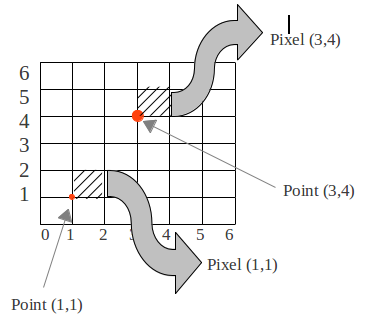
\includegraphics[scale=.8]{Files/Images/PixelAndPoint.png}
\end{figure}

Since we are going to deal with determining various geometrical shapes in this document we want to be clear how do we represent pixel throughout the book. Though there could be alternative ways of doing so, we would stick to the above method in the book.

\chapter{Breshenham Algorithm : Line}
\pagenumbering{arabic}
\section{Background}
It took me quite a while to appreciate the beauty of Brehsenham Line Drawing algorithm. Initially I thought It was just rounding off the decimal point to the nearest integer only in a zig-zag Barcelona way but to my fascination it turned out to be tremendously interesting yet very very finely simple.
 If two non-coincident points $(x_0,y_0)$and $(x_1,y_1)$ be given. The equation of line passing through these two points will be.
\begin{equation} \label{eq:basiceq}
	y=y_0+\frac{y_1-y_0}{x_1-x_0} (x-x_0)
\end{equation}
\begin{center}
	$y=y_0+\frac{\Delta y}{\Delta x} (x-x_0)$
\end{center}
\begin{center}
	$y=y_0+m (x-x_0)$
\end{center}
\begin{equation} \label{eq:stline}
	y=mx+ (y_0 -mx_0)
\end{equation}
Comparing equation \ref{eq:stline} with $y=mx+c$ we see
\begin{equation} \label{eq:valueofc}
	c=y_0-mx_0
\end{equation}

It is not difficult to see if two points  $(x_0,y_0)$ and $(x_1,y_1)$ are given then we can easily calculate the remaining points at any $x$ with the use of equation \ref{eq:basiceq} simply substuting value of $x$.
Let us think how do we calculate the points with a computer program. We would calculate the slope $m$ and $c$ then start a loop from $x_0$  with step $1$ and put value of $x$ in equation  \ref{eq:stline}  and simply find the values of $y$ corresponding to the value of $x$. 
The value of $m$  is generally a floating point number. Computer needs bit more labour to calculate the result of a floating point. Modern day VDU's are millions pixels in dimension. Just to draw a line across the VDU, poor CPU needs to do millions of floating point calculations which sucks more out of CPU. Lets fiddle around if we could somehow help the needy CPU here to avoid floating point multiplications.\\
\section{The Decision Parameter}
Lets first concentrate on special case where the slope of line $0 \leq m \leq 1$. If the first point is  $(x_0,y_0)$  and then with unit increase in the value of $x$ should increase $y$ by the value of slope $m$ which is less than 1. But $m$ is a floating point number, and the pixel coordinates are always integers. 
Let us assume that a intermediate point  $(x_k,y_k)$ is calculated already, the next point  $(x_{k+1},y_{k+1})$ is  either  $(x_k+1,y_k)$ or  $(x_k+1,y_k+1)$, (Note in both cases $x$ increases by just $1$).  If we could somehow decide which one between these two to  choose then our line would be known by induction. 
Let us find out which one of the integer is closer to the actual line. The actual coordinate of the line at $x_k+1$  is $y=m(x_k+1)+c$ The distance between the actual position from the two points to be decided are.
\begin{equation} \label{eq:dee1}
	d_1=[m(x_k+1)+c]-y_k
\end{equation}
\begin{equation} \label{eq:dee2}
	d_2=y_k+1-[m(x_k+1)+c]
\end{equation}


\begin{tabular}{l l}	
		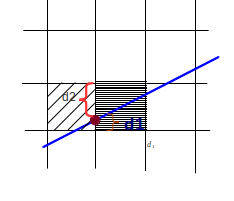
\includegraphics[scale=1]{Files/Images/DeeOne.png}	
		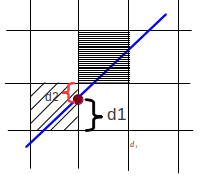
\includegraphics[scale=1.0]{Files/Images/DeeTwo.png}	\\
\end{tabular}
 
 The line crosses the ordinate at point below the mid point, which implies the lower pixel is nearer to line so the ordinate is not increased. But in the second case the actual line crosses the ordinate above the mid point which implies higher pixel is closer to line, so the ordinate is increased.\\
		
 
We will chose the next $y$ coordinate $y_k$ if $d_1 \leq d_2$ or else we will choose $y_k+1$.Subtracting equation \ref{eq:dee2} from equation \ref{eq:dee1} we get.
\begin{center}
	$d_1-d_2=[m(x_k+1)+c]-y_k-(y_k+1-[m(x_k+1)+c])$
\end{center}
\begin{equation} \label{eq:d1d2simplified}
	\Delta d=2mx_k-2y_k+2m+2c-1
\end{equation}
Here we are concentrating on line with slope $0\leq m \leq1$ so the value $(\Delta x = x_1-x_0)\geq 0$. so multiplying by $\Delta x$ on both sides of equation \ref{eq:d1d2simplified} preserves sign of $d_1-d_2$. Lets call this quantity $P_k$.
\begin{center}
	$P_k= \Delta x(2mx_k-2y_k+2m+2c-1)$
\end{center}
\begin{equation} \label{eq:simplifiedpk}
	\Rightarrow P_k=2\Delta yx_k-2\Delta xy_k+2\Delta y+\Delta x(2c-1)
\end{equation}

So, $\Delta d$ and  $P_k<0$ have the same sign. If $P_k<0$  we'll chose $(x_k+1,y_k)$ else  $(x_k+1,y_k+1)$ as the next point. 

\section{Recursive Relation Of Decision Parameter}
This expression above is the discriminant which decides which one between the two points in contention do we chose. For this reason $P_k$ is called the decision parameter. If $P_k$ determines the $k^{th}$ point then the next point is decided by $P_{k+1}$. Simply putting $k+1$ for $k$ in equation \ref{eq:simplifiedpk}  and keeping in mind that $x_{k+1}=x_k+1$ we get:
\begin{equation} \label{eq:pkplusone}
	P_{k+1}=2\Delta y(x_k+1)-2\Delta xy_{k+1}+2\Delta y+\Delta x(2c-1)
\end{equation}
Simplifying equation \ref{eq:pkplusone} and equation \ref{eq:simplifiedpk} we get:
\begin{equation} \label{eq:recursivep}
	P_{k+1}=P_k+2\Delta y-2\Delta x(y_{k+1}-y_k)
\end{equation}

We are down to just knowing the sign of $P_k$ to decide whether the next point after $(x_k,y_k)$ is $(x_k+1,y_k)$ or $(x_k+1,y_k+1)$ .

\begin{center}
	\begin{equation}
		y_{k+1}= \left\{
					\begin{array}{l l}
						y_k & \quad \text{if $P_k \leq 0$}\\
						y_k+1 & \quad \text{if $P_k>0$}
					\end{array}
				\right.
	\end{equation}
\end{center}

\section{Initial Decision Parameter}

The first point undoubtedly is $(x_0,y_0)$   but what is the first decision parameter? After first point $(x_0,y_0)$ is known we can know $P_0$. Simply put $(x_k,y_k)=(x_0,y_0)$ in equation \ref{eq:simplifiedpk}.
\begin{center}
	$P_0=2\Delta yx_0-2\Delta xy_0+2\Delta y+\Delta x(2c-1)$
\end{center}
Putting the value of $c$ from equation \ref{eq:valueofc}
\begin{center}
	$P_0=2\Delta yx_0-2\Delta xy_0+2\Delta y+\Delta x[2(y_0-mx_0)-1]$	
\end{center}
\begin{equation} \label{eq:initialp}
	\Rightarrow P_0=2\Delta y-\Delta x
\end{equation}
  
 
\section{Finding The Next Point}
So after $(x_0,y_0)$ is found, we can calculate $P_0$ by knowing value of $\Delta x$, $\Delta y$,$x_0$ and $y_0$. If $P_0\leq 0$ the next point is $(x_0+1,y_0)$ if $P_0>0$ the next point is $(x_1,y_1)=(x_0+1,y_0+1)$. So $P_0$ is calculated from $(x_0,y_0)$ and determines $(x_1,y_1)$ and so on. $P_k$ is calculated from $(x_k,y_k)$ and determines $(x_{k+1},y_{k+1})$ \\ 
Summarizing this:
\begin{center}
\begin{equation}
	y_1 = \left\{
				\begin{array}{l l}
					y_0 & \quad \text{if $P_0\leq 0$ }\\
					y_0+1 & \quad \text{if $P_0>0$ }
				\end{array} 
		\right.
\end{equation}
\end{center} 
Putting $k=0$ in equation \ref{eq:recursivep} we get:
\begin{center}
	$P_1=P_0+2\Delta y-2\Delta x (y_1-y_0)$
\end{center}

Which determines $(x_2,y_2)$ and so on.. and hence all the points of the line.

\section{The Breshenham Algorithm}
Writing out algorithm for this:
%\begin{enumerate}
%	\item \quad Get the end points$(x_0,y_0)$ and$(x_1,y_1)$ calculate$\Delta x$ and$\Delta y$ and hence $P=P_0$ 
%	\item \quad Initial point $(x,y)=(x_0,y_0)$and \\
%	\quad Begin := 
%	\item \qquad Plot $(x,y)$
%	\item \qquad Store previous $y : t \leftarrow y$ .
%	\item \qquad if $P>0$ then $y \leftarrow y+1$
%	\item \qquad Update$P \leftarrow P+2\Delta y -2\Delta x(y-t)$ from equation \ref{eq:recursivep} above.
%	\item \qquad Increase $x \leftarrow x+1$.
%	\item \quad Loop while $x\leq y$ 
%\end{enumerate}

\begin{algorithm}[H]
		
	\SetAlgoLined
	\KwData{ Get end points $(x_0,y_0)$ $(x_1,y_1)$}
	$P=2\Delta y-\Delta x$\;
	$(x,y)=(x_0,y_0)$\;
	\While{$x\leq y$}{
		Plot$(x,y)$\;
		$t \gets y$\;

		\If{$P\geq 0$}{
			$y\gets y+1$\;
		}
		$P \gets P+2\Delta y -2\Delta x(y-t) $\;
		$x\gets x+1$\;
	}
	\caption{Breshenham Line Algorithm for $0 \leq m  \leq 1$}
\end{algorithm}


\section{Lines With Any Slope}

But line in real life are never always restricted to have the slope  $0\leq m\leq 1$  . How can we extend this method to find the points of line in all the situation where the value of slope may be any number from the real axis?

Ok, lets begin the ride.

Lets us divide the Cartesian plane into 8 equal octant. The lines with slope with multiples of $\frac{\pi}{4}$ will suffice our division of the planes into octant. From our journey so far we have completed the calculation of points of line anywhere in the first octant. Now the job is to conquer the rest of the octant. There is a nice symmetry between the rest of the octant with the first. There exist a unique transformation matrix that transforms the line back and forth between first and the rest octant. Now the job is almost over. 
Identify the octant and transform it to first octant, calculate the points with the artifice we have done so far, and transform back to the original octant to plot.
Bravo!! we conquered Everest.\\
Lets do the mathematics of the idea then.
\subsection{Finding The Octant}
Let us, for our ease, transform the co-ordinate system with axes parallel but the origin transferred to the initial point of line. We do this because we would not then have to worry about two points to determine a line, only the final point would describe the line completely as the first point will be the origin of our new coordinate system. 
It is easy to determine the octant, as we have divided above, which the line lies in, simply by finding out which octant the final point lies in. 

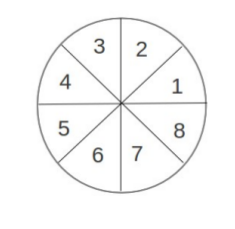
\includegraphics[scale=1.0]{Files/Images/OctantNumbered.png}
If the $x$ coordinate is positive there are four candidate for the octant namely 1,2,8,7. Among these four the candidates are down to 1 and 2 if the $y$ coordinate is +ve as well. And whether the $y$ coordinate is greater than $x$ determines whether the line lies on 2nd quadrant or first. Similarly the rest of the octants are determined. 

The table below shows how to figure how the octant of the line with the coordinate of the end point.

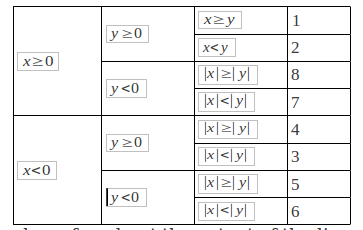
\includegraphics[scale=1.0]{Files/Images/FindingOctant.png}



\subsection{The Transformation Matrix}
After we have found out the octant of the line with this. Our task is transform every line into first octant then find the corresponding points on first octant and transform back to original octant to plot.
What transforms the points back and forth between the given octant and the octant number 1. All the points are transformed to first octant where the coordinate of the point is $(x,y)$

  
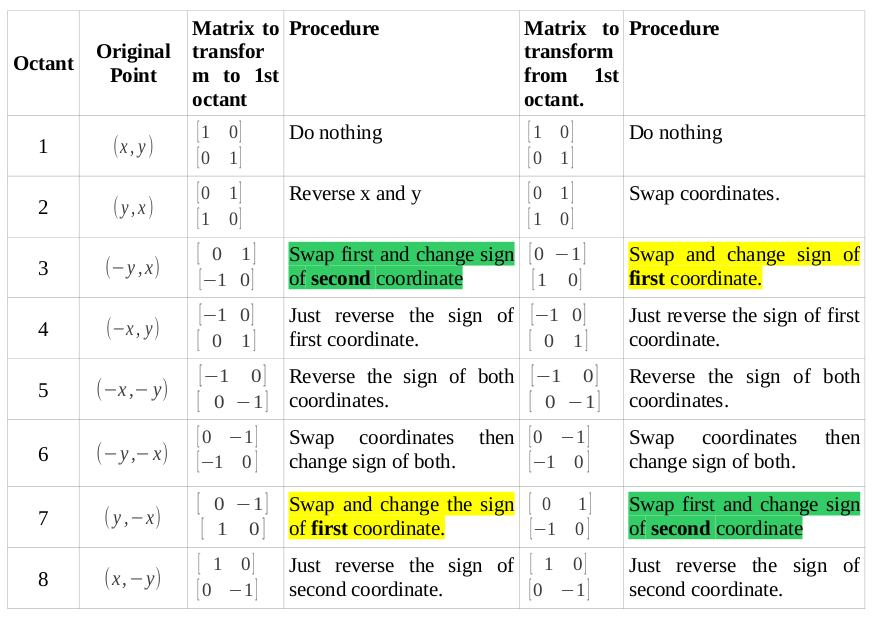
\includegraphics[scale=0.50]{Files/Images/Matrix.png}

From above table we see that same matrix transforms back and forth between all the octants except for octant number 3 and 7. It seems that we have to keep track of whether we are transferring from octant 3 to 1 or 1 to 3. And similarly for octant 7. 

We can do this by using one transformation to transform from given octant to the first. And the other to transform from 1st to the given octant. For all but 3 and 7 both the transformation would be same.  Just two of these odd octants are trying to force us to make two transformations for the well behaved 6 of the rest. Can we get over the odds??
Luckily yes.
We get  extremely lucky here, there is a symmetry between the odd ones. Once the point is transferred from 3rd to the 1st octant the point transforms back to 3rd octant exactly as the point is transferred from 7th to the first. And also once the point is transferred from 7th to 1st octant the point transfers back to the 7th octant exactly as the point is transferred from 3rd to 1st.
Lets go fooling around. First transfrom the point normally from the given octant. If the octant is one of 7 or 3 then fool the system by changing the octant index  to 3 or 7 respectively. Then do normally.

\section{Implementation On C++}
Below is a computer program written in C++ implementing the algorithm.

\begin{scriptsize}
	\lstinputlisting[language=C++]{./Files/SourceCode/Line.cpp}
\end{scriptsize}

\chapter{Breshenham Algorithm : Circle}
\section{Definition}

 A \emph{circle} is locus of a moving point which moves such that it's distance from a fixed point-called center- is always constant- called the radius. This is the basic definition of circle which completely describes a circle. 
\section{Equation of Circle}
The most well known equation of a circle which uses the above definition is:
\begin{equation} \label{eq:generalcircle}
	(x-x_0)^2+(y-y_0)^2=r^2
\end{equation}
where $(x_0,y_0)$ is the coordinate of the center and $r$ is the radius of the circle. if $(0,0)$ is the center of the circle the equation reduces to:
\begin{equation} \label{eq:origincircle}
	x^2+y^2=r^2
\end{equation} 

Circle can be mathematically known with other equations as well. The parametric equation of a circle are:
\begin{equation}
	x=r\cos\theta
\end{equation}
\begin{equation}
	y=r\sin\theta
\end{equation}

If our task is to find the points of circle with given center and radius, we would be more inclined to use the relation \ref{eq:origincircle}. Simplifying it.
\begin{equation}
	y=\sqrt{r^2-x^2}
\end{equation}
 Using this equation we can find the value of $y$ for any given value of $x$. For reasons mentioned earlier we would rather not ask CPU to work this equation out for long. There has to be some way. Let's find the way.
 \section{Two Possible Points}
 With the process mentioned earlier, lets again divide the plane into 8 octants. Assuming the circle is centered at origin and given radius $r$ lets find points of the  lying in the second octant,(octant divided as in the figure in the previous chapter). We begin with the known point on the second octant $(0,r)$. Then for the $2^{nd}$ octant the slope of tangent to the circle is between $\leq \vert m \vert \leq 1$ or $-1\leq m \leq 0$. So with unit increase in $x$ coordinate the y coordinate just decreases approximately by slope at that point. But we have are in advantage of knowing that the slope is not less than 1. So the $y$ coordinate doesn't fall by more than one. So we could safely say if $(x_k,y_k)$ is a intermediate point in the second octant, the next point is either  $(x_k+1,y_k)$ or $(x_k+1,y_k-1)$. Notice since the slope is negative the $y$ coordinate falls, contrary to line on the first octant. We are finally down just between two points to figure out the entire circle by induction. If somehow we could figure out which one between these points to chose then our circle would be known completely. 
 \section{The Decision Parameter}
 
 Let's restate the equation of circle once again this time rather differently. Lets call it a circle function.
 \begin{equation} \label{eq:circlefunction}
 	f(x,y)=x^2+y^2-r^2
 \end{equation}
  If any point satisfies the circle function then the point lies exactly on the locus. But what happens if it doesn't satisfy? The resulting quantity will be either positive or negative if it doesn't satisfy. If the result  is positive then the point lies on the outside of the circle or else inside (area enclosed by circle) the circle.\\
  Let us now suppose that an intermediate point $(x_k,y_k)$ has been determined. The next point  $(x_{k+1},y_{k+1})$ from above discussion is either$(x_k+1,y_k)$ or $ (x_k+1,y_k-1)$. Lets decide which one between them do we chose. Having determined current point.\\
   If we put the current point on the circle function, it only tells whether the current point is inside or outside the circle, and tells nothing more about next point. One way is to test whether the point $(x_k+1,y_k)$ lies inside the circle. But the better point to test would be $(x_k+1,y_k-\frac{1}{2})$, the point midway between the points of contention, because if this point lies outside the circle, then the circle would be closer to the point $(x_k+1,y_k-1)$ and if it lies inside, the circle  would be closer the point $(x_k+1,y_k)$ for our idea is to select the closest integer approximation of the actual circle ordinate.\\
   Putting $(x_k+1,y_k-\frac{1}{2})$ in equation \ref{eq:circlefunction} we get:
\begin{equation} \label{eq:decisioncircle}
	P_k=f(x_k+1,y_k-\frac{1}{2})=(x_k+1)^2+(y_k-\frac{1}{2})^2-r^2
\end{equation}
If this comes out to be positive the point midway between the points of contention $(x_k+1,y_k-\frac{1}{2})$ lies outside the circle suggesting $(x_k+1,y_k-1)$ lies closer to the circle or else if it comes negative the point $(x_k+1,y_k)$ lies closer to the actual circle. 
 \begin{center}
	\begin{equation}
		y_{k+1}= \left\{
					\begin{array}{l l}
						y_k & \quad \text{if $P_k \leq 0$}\\
						y_k-1 & \quad \text{if $P_k>0$}
					\end{array}
				\right.
	\end{equation}
\end{center}
 
  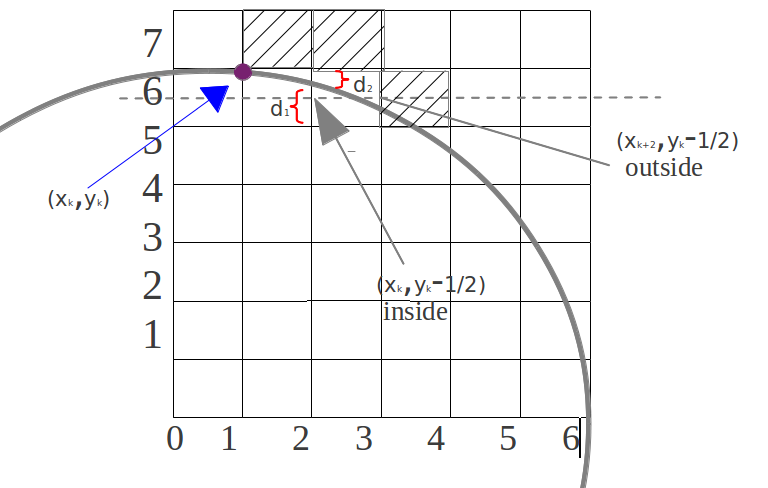
\includegraphics[scale=0.50]{Files/Images/CirclePoint.png}
\section{Recursive Relation Of Decision Parameter}
For quite obvious reasons from our discussion of previous chapter, we would like to have a recursive relation of decision parameter $P_k$. Putting $k+1$ for $k$ in equation \ref{eq:decisioncircle}.
\begin{equation} \label{eq:decisioncircle2}
	P_{k+1}=(x_k+2)^2+\left(y_{k+1}-\frac{1}{2}\right)^2-r^2
\end{equation}
Subtracting equation \ref{eq:decisioncircle} from equation \ref{eq:decisioncircle2} we get.
\begin{equation} \label{eq:circlerecursivep}
	P_{k+1}=P_k+2x_k+(y_{k+1}^2-y_k^2)-(y_{k+1}-y_k)+3
\end{equation}
 Which is the decision parameter for a circle.
 \section{Initial Decision Parameter}
 Now obviously, since we are starting from point on second octant $(0,r)$ is the first point we chose. Therefore $(x_0,y_0)=(0,r)$. Putting $k=0$ in equation \ref{eq:decisioncircle} we get.
 \begin{center}
 	$P_0=(x_0+1)^2+(y_0-\frac{1}{2})^2-r^2$\\
	$=(0+1)^2+(r-\frac{1}{2})^2-r^2$ 	
 \end{center}
 \begin{equation} \label{eq:p0circle}
	P_0=\frac{5}{4}-r
 \end{equation}
 This is a tidy initial decision parameter.\\

 \section{The Breshenham Algorithm}
Writing out algorithm for this:

%\begin{enumerate}
%	\item \quad Get the radius $r$ and center $(h,k)$calculate $P=P_0=5/4-r$ 
%	\item \quad Initial point $(x,y)=(0,r)$and \\
%	\quad Begin := 
%	\item \qquad Plot $(h+x,k+y)$
%	\item \qquad Store previous $y : t \leftarrow y$ .
%	\item \qquad if $P>0$ then $y \leftarrow y-1$
%	\item \qquad Update$P \leftarrow P+2x+(y^2-t^2)-(y-t)+3$ from equation \ref{eq:circlerecursivep} above.
%	\item \qquad Increase $x \leftarrow x+1$.
%	\item \quad Loop while $x\leq y$ 
%\end{enumerate}
\begin{algorithm}[H]
		
	\SetAlgoLined
	\KwData{ Get radius $r$ and center $(h,k)$}
	$P\gets 5/4-r$\;
	$(x,y) \gets (x_0,y_0)$\;
	\While{$x\leq y$}{
		Plot$(x+h,y+k)$\;
		$t \gets y$\;

		\If{$P\geq 0$}{
			$y\gets y-1$\;
		}
		$P \gets P+2x+(y^2-t^2)-(y-t)+3 $\;
		$x\gets x+1$\;
	}
	\caption{Mid Point Circle Algorithm}
\end{algorithm}

.\\[.2cm]

Compare it with the breshenham algorithm for the straight line and get amazed. The algorithm is exactly the same. Only the formula for the decision parameter are different.\\

  For a circle, there is radial symmetry. This symmetry allows us determine the circle completely just by knowing the points of just the first octant. We would implement this process until $x_k\leq y_k$ which indicates the point lies on the second octant. For a point $(x,y)$, its transformation to the rest of the octant also are the closest points of the circle. So, for $(x,y)$ lying on second octant $(y,x)$ lies on  first octant. And also for the rest of octant find the transformed point and plot it.

\section{Implementation in C++}
Breshenham Circle Drawing Algorithm adopted in a program  in C++.
\lstinputlisting[language=C++]{./Files/SourceCode/Circle.cpp}
\chapter{The Breshenham Algorithm : Ellipse}
\section{Defintion}
An ellipse is the locus of a point which moves such that the ratio of its distance from a fixed point( called the focus) and a straight line (called the directrix) is always constant, the constant is called the eccentricity of the ellipse and is less than one. If the eccentricity is greater than one the locus would be a hyperbola. Ellipse is a closed curved.\\
Another equivalent definition which also gives us ellipse is that, ellipse is the locus of moving point whose sum of distances from two points called the foci is always constant. Both these definition are just two different demonstration of the same geometrical shape and are interchangeable. 
\section{Equation of Ellipse}
We would not go into the mathematical details of the ellipse but rather we will ask a few equations from the mathematician and state the equation of ellipse as they provide us.
\begin{equation} \label{eq:generalellipse}
	\frac{x^2}{a^2}+\frac{y^2}{b^2}=1
\end{equation}
Above equation can be modified into a different form as:
\begin{center}
	$b^2x^2+a^2y^2-a^2b^2=0$
\end{center}

If we had to determine the points to plot in a graph or to disply in a vdu we would rather like the equation that gives the value of $y$ coordinate for corresponding value of $x$ coordinates. Making $y$ as a function of $x$ from above relation we get:
\begin{equation}
	y=\frac{b}{a}\sqrt{a^2-x^2}
\end{equation}
To work out this formula we need to do lots of calculation as square of a floating point number, fractions, their product and tedious square root.\\
There is another equation as well called the polar equation of the ellipse.
\begin{equation}
	r=\frac{l}{1+\epsilon cos(\theta)}
\end{equation}
 For reasons mentioned earlier we would like to have a simpler process to find out the points of an ellipse.

 \section{Two Parts on Quardrant}
 

 Unlike a circle, the ellipse doesn't posses one symmetry of reflection on the line $y=x$. So as in circle we cant just calculate point on a single octant and reflect on other octants to plot. We certainly would exploit the symmetry along the axes but we have first to determine all point on one of the quardrants so they can be transformed to other quardants. But for our misery the slope of tangent to ellipse on the first quardrant takes all values from zero to infinity. But so far we have used Breshenham algorithm with one commong thing(in line and circle) in mind, the solpe had the property.$0 \leq \vert m \vert \leq 1$ or $-1\leq m \leq 0$. \\
 The ellipse doesn't posses symmetry in the octant and doesn't have the required property, so we are in deep deep trouble. What do we do now??\\
 Don't panic just yet. Lets go for yet another  trickery again.\\

Keeping in mind that we will exploit the property $0 \leq \vert m \vert \leq 1$ or $-1\leq m \leq 0$.  Lets divide the ellipse on the first quardrant into two parts, one part of which has the slope of tangent exaclty between $0 \leq \vert m \vert \leq 1$, Starting from $(0,b)$ where the slope is 0, the slope decreases and reaches -1 at ceratin point. Lets find that point.\\
To find the point lets find the slope of tangent to the ellipse. Differentiating equation \ref{eq:generalellipse} we get

\begin{center}
	$\frac{dy}{dx}=-\frac{b^2x}{a^2y} $
\end{center}
The for the slope to be greater than -1 we must have.
\begin{center}
	$\frac{dy}{dx}\geq -1$\\
	$\Rightarrow -\frac{b^2x}{a^2y} \geq -1$
\end{center}
\begin{equation} \label{eq:firstpartmarker}
	\Rightarrow b^2x\leq a^2y
\end{equation}
equation \ref{eq:firstpartmarker} must be satisfied for the slope at that point to be $0 \leq \vert m \vert \leq 1$

\section{The Two Points} 
   Assuming the ellipse is centered at origin and given semi major axis $a$ and semi minor axis $b$ lets find points of the  lying in the first part of the first quardrant,. \\ \\
   We begin with the known point on the second octant $(0,b)$. Then for the first part in the first quardrant the slope of tangent to the ellipse is between $0 \leq \vert m \vert \leq 1$ or $-1\leq m \leq 0$. So with unit increase in $x$ coordinate the y coordinate just decreases approximately by slope at that point. But we have are in advantage of knowing that absolute value of the slope is not less than 1. So the $y$ coordinate doesn't fall by more than one. So we could safely say if $(x_k,y_k)$ is a intermediate point in the first part of first quardrant, the next point is either  $(x_k+1,y_k)$ or $(x_k+1,y_k-1)$. Notice since the slope is negative the $y$ coordinate falls, contrary to line on the first octant but similar to the circle. We are finally down just between two points to figure out the entire ellipse by induction. \\ \\
   If somehow we could figure out which one between these points to chose then our ellipse would be known completely. 

\section{The Decision Parameter}
Lets again mention the equation of ellipse but this time rather differently. Lets call it an ellipse function.
\begin{equation} \label{eq:ellipsefunction}
	f(x,y)=bx^2+ay^2-a^2b^2
\end{equation}

Any point satisfying this equation lies on the ellipse and any other point not satisfying lies either inside the ellipse or outside teh ellipse as an ellipse is a geometrically closed curve.\\
When a point substituted in this function gives a negative value the point lies inside the ellipse and when the point gives positive value then the point lies outside the ellipse.\\
 Let us now suppose that an intermediate point $(x_k,y_k)$ has been determined. The next point  $(x_{k+1},y_{k+1})$ from above discussion is either$(x_k+1,y_k)$ or $ (x_k+1,y_k-1)$. Lets decide which one between them do we choose having determined current point.\\
  \\ Similar to the discussion made for circle, If we put the current point on the ellipse function, it only tells whether the current point is inside or outside the ellipse, and tells nothing more about next point. One way is to test whether the point $(x_k+1,y_k)$ lies inside the ellipse. But the better point to test would be $(x_k+1,y_k-\frac{1}{2})$, the point midway between the points of contention, because if this point lies outside the ellipse, then the ellipse would be closer to the point $(x_k+1,y_k-1)$ and if it lies inside, the ellipse  would be closer the point $(x_k+1,y_k)$ for our idea is to select the closest integer approximation of the actual ellipse ordinate.\\
   Putting $(x_k+1,y_k-\frac{1}{2})$ in equation \ref{eq:ellipsefunction} we get:
\begin{equation} \label{eq:decisionellipse}
	P_k=f(x_k+1,y_k-\frac{1}{2})=b^2(x_k+1)^2+a^2(y_k-\frac{1}{2})^2-a^2b^2
\end{equation}
If this comes out to be positive the point midway between the points of contention $(x_k+1,y_k-\frac{1}{2})$ lies outside the ellipse suggesting $(x_k+1,y_k-1)$ lies closer to the ellipse or else if it comes negative the point $(x_k+1,y_k)$ lies closer to the actual ellipse
 \begin{center}
	\begin{equation}
		y_{k+1}= \left\{
					\begin{array}{l l}
						y_k & \quad \text{if $P_k \leq 0$}\\
						y_k-1 & \quad \text{if $P_k>0$}
					\end{array}
				\right.
	\end{equation}
\end{center}

\section{Recursive Relation Of Decision Parameter}
For quite obvious reasons from our discussion of previous chapter, we would like to have a recursive relation of decision parameter $P_k$. Putting $k+1$ for $k$ in equation \ref{eq:decisionellipse}.
\begin{equation} \label{eq:decisionellipse2}
	P_{k+1}=a^2(x_k+2)^2+b^2(y_{k+1}-\frac{1}{2})^2-a^2b^2
\end{equation}
Subtracting equation \ref{eq:decisionellipse} from equation \ref{eq:decisionellipse2} we get.
\begin{equation} \label{eq:ellipserecursivep}
	P_{k+1}=P_k+2b^2x_k+a^2(y_{k+1}+y_k-1)(y_{k+1}-y_k)+b^2
\end{equation}
 Which is the decision parameter for an ellipse.
 \section{Initial Decision Parameter}
 Now obviously, since we are starting from point  $(0,b)$ is the first point we chose. Therefore $(x_0,y_0)=(0,b)$. Putting $k=0$ in equation \ref{eq:decisionellipse} we get.
 \begin{center}
 	$P_0=b^2(x_0+1)^2+a^2(y_0-\frac{1}{2})^2-a^2b^2$\\
	$=b^2(0+1)^2+a^2(b-\frac{1}{2})^2-a^2b^2$ 	
 \end{center}
 \begin{equation} \label{eq:p0ellipse}
	P_0=b^2-a^2b+\frac{a^2}{4}
 \end{equation}
 This is a again neat and tidy initial decision parameter.\\

 \section{The Breshenham Algorithm}
Writing out algorithm for this:
%\begin{enumerate}
%	\item \quad Get the semi major axis  $a$  and semi minor axis $b$ and center $(h,k)$calculate $P_0=b^2-a^2b+\frac{a^2}{4}$ 
%	\item \quad Initial point $(x,y)=(0,b)$and \\
%	\quad Begin := 
%	\item \qquad Plot $(h+x,k+y)$
%	\item \qquad Store previous $y : t \leftarrow y$ .
%	\item \qquad if $P>0$ then $y \leftarrow y-1$
%	\item \qquad Update$P \leftarrow P+2b^2x+a^2(y+t-1)(y-t)+b^2$ from equation \ref{eq:ellipserecursivep} above.
%	\item \qquad Increase $x \leftarrow x+1$.
%	\item \quad Loop while $b^2x\leq a^2y$ 
%\end{enumerate}

\begin{algorithm}[H]
		
	\SetAlgoLined
	\KwData{ Get semi major axis $a$ and semi minor axis and $b$  center $(h,k)$}
	$P\gets b^2-a^2b+a^2/4$\;
	$(x,y) \gets (0,b)$\;
	\While{$b^2x\leq a^2y$}{
		Plot$(x+h,y+k)$\;
		$t \gets y$\;

		\If{$P\geq 0$}{
			$y\gets y-1$\;
		}
		$P \gets P+2b^2x+a^2(y+t-1)(y-t)+b^2 $\;
		$x\gets x+1$\;
	}
	\caption{Mid Point Ellipse Algorithm}
\end{algorithm}
.\\[.5cm]
\linebreak
Compare it with the breshenham algorithm for the straight line and circle and get even more amazed. The algorithm is exactly the same. Only the formula for the decision parameter are different.\\

\section{All the points}
Equipped with above arms we can calculate the points of ellipse on first part of first quardrant. We would like then to find the points on the second quardrant. The idea is, get the points of first part first. Then swap the semi major and semi minor axis. Find the points for the swapped ellipse. Then swap back the calculated points. With this simple artifice we can find points on the second art as well. \\
Now we have completed the ellipse in the first quardrant. To find points on other quardrant explioit the axial symmetry and transform the points to rest of the three quardrants as well. Our ellipse is then ready. Nice and tidy.



\section{Implementaion On C++}
\lstinputlisting[language=C++]{./Files/SourceCode/Ellipse.cpp}


\end{document}

